% !TEX root =../thesis.tex
\chapter{Automatic fitting of optical Type Ia Supernova spectra - the DALEK project}
\label{chap:dalek}

The last chapters (Chapters \ref{chap:sn1572_starg, chap:sn1572_hires, chap:sn1006_flames} were dedicated to the hunt for donor stars and did not use the measurements from the \snia-phenomenon itself. In this chapter we will describe the extraction of yields and energies from optical spectra. 

The two main sources of information in spectra, are the spectra themselves as well as their time evolution. There have been a few attempts to extract the details of the stellar explosions from one or two of these sources. All of them employ the technique of fitting the spectra using synthetic spectra. One of the main parts is the radiative transfer program that creates the synthetic spectra. There are several different radiative transfer-codes in the community. 


\cite{2000PhDT.........6F} wrote a very simple radiative transfer code called \synow. \synow is a highly parametrized code and thus is mainly used for line identification rather than actual fitting of supernova spectra. It runs 
The main code (henceforth \mlc) used in this work is an evolved code of  \cite{1993A&A...279..447M, 2000A&A...363..705M}. Compared to the \synow-code the \mlc-code calculates a radiative equlibirum tepmerature and uses this to compute internally consistent ionization ratios. In addition \mlc takes electron scattering into account as well as allowing for photon branching. 


Codes such as PHOENIX\cite{1999JCoAM.109...41H}, SEDONA \cite{2006ApJ...651..366K} and ARTIS \cite{2009MNRAS.398.1809K} are powerful 3D radiative transfer codes. They are the most "physical" codes available but take hours on supercomputers to produce spectra. These codes, however, are not feasible for fitting observed spectra as they take too long for each iteration. 

The main aim of this work was to automatically fit the torrent of observed spectra expected from the next generation of supernova searches. We opted to use the \mlc-code  as it provides a good compromise between speed and "realism".

In section \ref{sec:mlc_intro}we will introduce a the inner-workings of the \mlc-code.  We will discuss the properties of the search space in \ref{sec:searchspace} and will introduce our optimisation strategies in \ref{sec:optimisation_strategies}. Finally we will conclude and give an outlook over future work for this unfinished project in section \ref{sec:dalek_conclusion}.

\section{The \mlc-Code}

The supernova can be divided in two different phases: the photospheric phase and the nebular phase. The \mlc-code only models the photospheric phase.
In this photospheric phase the supernova is treated like a sharp photosphere emitting a black-body spectrum with a fast moving layer of ejecta above that. The ejecta is assumed in homologous expansion, which means that the velocity is a linear function of the radius:
\[
	v=  r / t.
\]
One major assumption that the code makes is that of the Sobolev approximation. This means that at the interaction between photon and line resonance happens only at one specific point (thus disregarding any broadening effects to the line). For example a photon in free flight from the photosphere will be able to interact with resonance lines of lower and lower frequencies. 
There are two main caveats ??? supernova wind fast enough so lines don't blend ??? temperature to high ????

In the simplest case we can treat the ejecta as homogeneous in temperature and abundance. For now we will also assume a pure scattering line interaction. This means that the photon is absorbed at a resonance frequency and then instantaneously reemitted with the same frequency into a random direction. This in in contrast to photon branching which we will discuss later. 

We assume a time since explosion $t_e$, a photospheric velocity \vph and \teff of the photosphere. 
In the first instance the photon is emitted with a random frequency and a random angle drawn from a Blackbody distribution $B(\teff)$.  



\section{Properties of Type Ia supernova spectra}

When fitting manually there are several features that help guide the direction of the fit. We will attempt to explain by using a spectrum of SN2002bo (cite?????) 10 days before maximum. In this section we will only talk about fits with no abundance stratification. Stephan Hachinger has kindly provided his manually obtained best fitting parameters ( for the supernova at this stage (see Figure \ref{fig:sn2002bo-10_bf}).

\begin{figure}[htbp] %  figure placement: here, top, bottom, or page
   \centering
   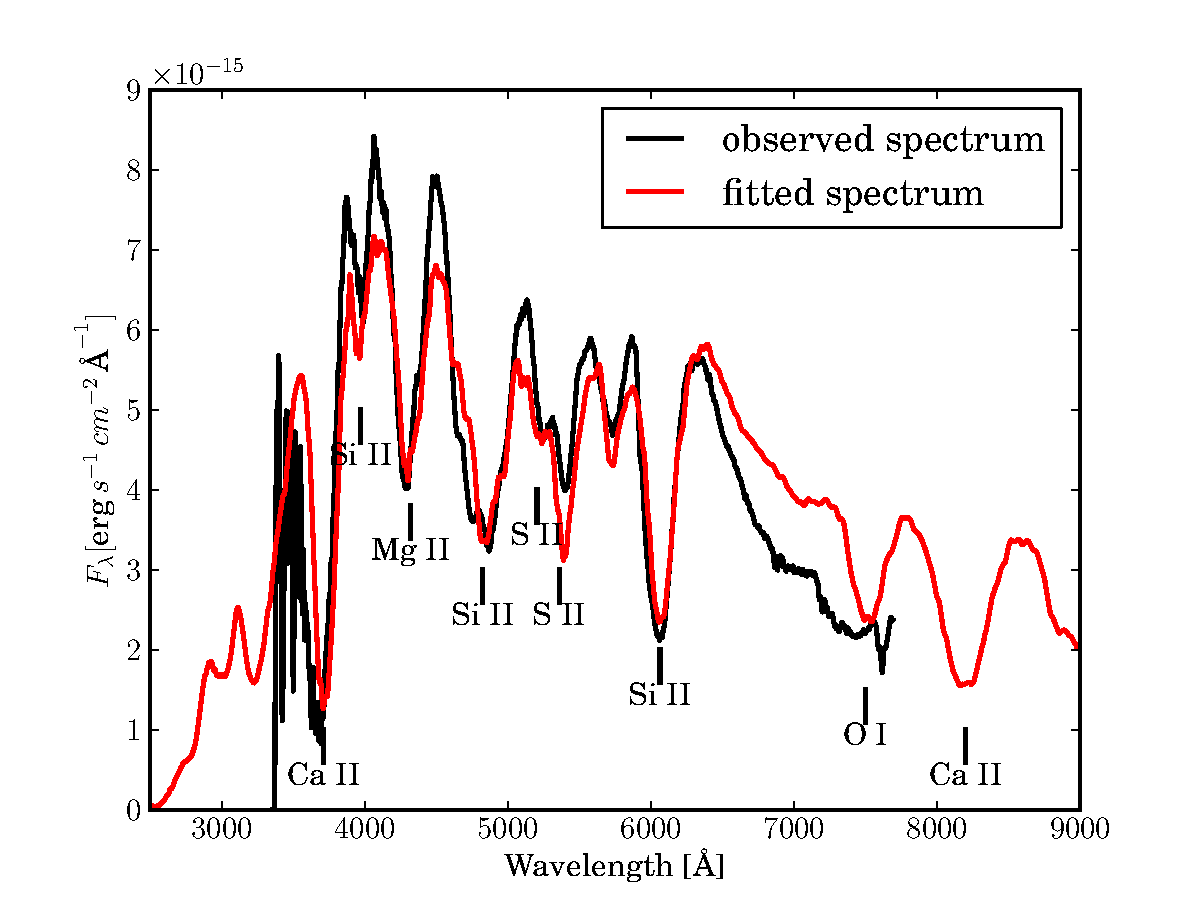
\includegraphics[width=\textwidth]{chapter5/plots/bf2002bo-10.pdf} 
   \caption{example caption}
   \label{fig:sn2002bo-10_bf}
\end{figure}

The chosen fundamental parameters are $\loglbol=xx$, $\vph=xxx$. We have listed the non-zero abundances in Table{tab:sn2002bo_perf_param}. 

The P-Cygni profiles of many features are easily visible. The Calcium line in the blue can be seen to be to blueshifted in relation to the model. This property is not unusual and is thought to come from high velocity component at the outer edge of the ejecta. The next major known discrepancy that can be seen is the excess of flux redwards of  $\approx 6200 \AA$.  This is a region that usually does not fit well as the underlying black body spectrum overestimates the flux in this region. When fitting manually often one tries to fit the depth the lines instead of the continuum.

A large offset in \lum\ is easily visible as a large offset of the continuum. Thus it is easy to constrain the parameter space in \lum\ initially. \lum\ also has influence on the temperature of the model through:
\[
L_{\rm bol} = 4\pi\sigma\, R^2\,T^4 = 4\pi\sigma\,\vph\,\texp.
\label{eq:Lum_temp_relation}
\]









